\documentclass[../lecture1-variables.tex]{subfiles}

\begin{document}

\section{Programming Challenge}

% -------------------------------------------------------------------

\begin{frame}[fragile]{Calculator Challenge}
    The following program should function as a basic calculator; it should ask
    the user to input what type of arithmetic operation he would like, and then
    ask for the numbers on which the operation should be performed. The calculator
    should then give the output of the operation.
\end{frame}

\begin{frame}[fragile]{Calculator Challenge Problem Code}
    \begin{cppcode}[]
         <iostream>

___ multiply(int x, int y)
{
    ______ x _ y;
}

____ divide(int x, int y)
{
    _____ x _ y;
}

_____ add(int x, int y)
{
    ______ x _ y;
}

______ subtract(int x, int y)
{
    _____ x _ y;
}

using namespace std;

___ _____()
{
    ____ op = 'c';
    ____ x, y;
    while(op! = 'e')
    {
        cout __ "What operation would you like to perform:";
        cout __ "add(+), subtract(-), divide(/), multiply(*), [e]xit?";
        cin __ op;
        switch(op)
        {
            case '+':
                cin __ x;
                cin __ y;
                cout __ x __ "+" __ y __ "=" __ add(x, y) __ endl;
                break;
            case '-'_
                cin __ x;
                cin __ y;
                cout __ x __ "-" __ y __ "=" __ subtract(x, y) __ endl;
                break;
            case '/':
                cin __ x;
                cin __ y;
                cout __ x __ "/" __ y __ "=" __ divide(x, y) __ endl;
                break;
            case '*':
                cin __ x;
                cin __ y;
                cout __ x __ "*" __ y __ "=" __ multiply(x, y) __ endl;
                break;
            case 'e':
                break;
            ______:
                cout __ "Sorry, try again" __ endl;
        }
    }

    return _;
}
    \end{cppcode}
\end{frame}

\begin{frame}[fragile]{Calculator Challenge Solution Code}
    \begin{cppcode}[]
#include <iostream>

int multiply(int x, int y)
{
    return x * y;
}

int divide(int x, int y)
{
    return x / y;
}

int add(int x, int y)
{
    return x + y;
}

int subtract(int x, int y)
{
    return x - y;
}

using namespace std;

int main()
{
    char op = 'c';
    int x, y;

    while(op != 'e')
    {
        cout << "What operation would you like to perform:";
        cout << "add(+), subtract(-), divide(/), multiply(*), [e]xit?";
        cin >> op;

        switch(op)
        {
            case '+':
                cin >> x;
                cin >> y;

                cout << x << "+" << y << "=" << add(x, y) << endl;
                break;
            case '-':
                cin >> x;
                cin >> y;

                cout << x << "-" << y << "=" << subtract(x, y) << endl;
                break;
            case '/':
                cin >> x;
                cin >> y;

                cout << x << "/" << y << "=" << divide(x, y) << endl;
                break;
            case '*':
                cin >> x;
                cin >> y;

                cout << x << "*" << y << "=" << multiply(x, y) << endl;
                break;
            case 'e':
                break;
            default:
                cout << "Sorry, try again" << endl;
                break;
        }
    }

    return 0;
}
    \end{cppcode}
\end{frame}

% -------------------------------------------------------------------

\begin{frame}[fragile]{Check this out}
    \begin{center}
        \makebox[\textwidth]{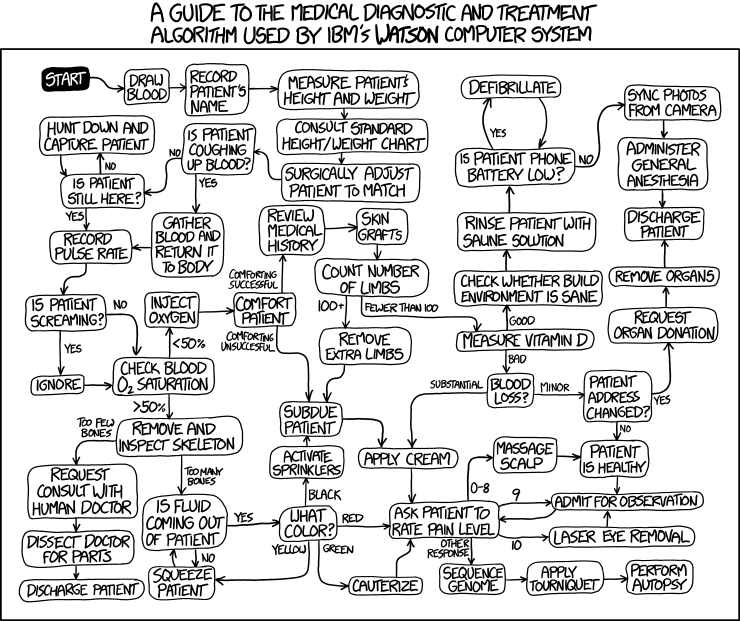
\includegraphics[width=\paperwidth,height=\textheight,keepaspectratio]{graphics/xkcd1619-watson_medical_algorithm.png}}
    \end{center}
\end{frame}

% -------------------------------------------------------------------

\end{document}
